\subsection{Network Layer}

The network layer works on top of the neighbor to neighbor layer which implements reliable neighbor to neighbor transmission. The network packet structure is shown in the figure \ref{fig:network_packet} where the first byte indicates the length of the packet, the second is used for communication dependent flags, the packet ID byte is a unique ID for each packet, the Source ID byte refers to the ID of the module sending the message, the Dest ID byte is used to identify the ID of the module where the packet has been sent to, the Command byte is the command (passed to the application layer) which the destined module will do and finally the $Data[0] \ldots Data[n]$ bytes are bytes associated to the command that is going to be done.

\begin{figure}[htb]
\centering
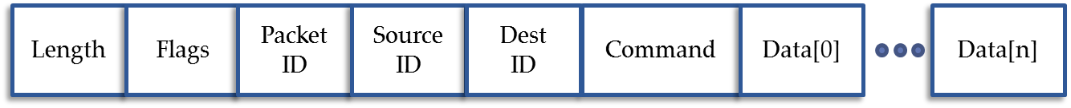
\includegraphics[width=0.8\textwidth]{figures/network_packet.png}
\caption{Network Packet}
\label{fig:network_packet}
\end{figure}

If a module that wants to send a message to another module, it first construct the packet setting the appropriate flags and structure, then it broadcasts the message to every module attached to it and the waits for an acknowledgment back from the module it sent the message to. If no acknowledgment is received it tries a fixed (configurable) amount of times to send the message and then fails if it still does not receive an acknowledgment back. The figure \ref{fig:sending_algorithm} shows the algorithm for sending a network message.

\begin{figure}[htb]
\centering
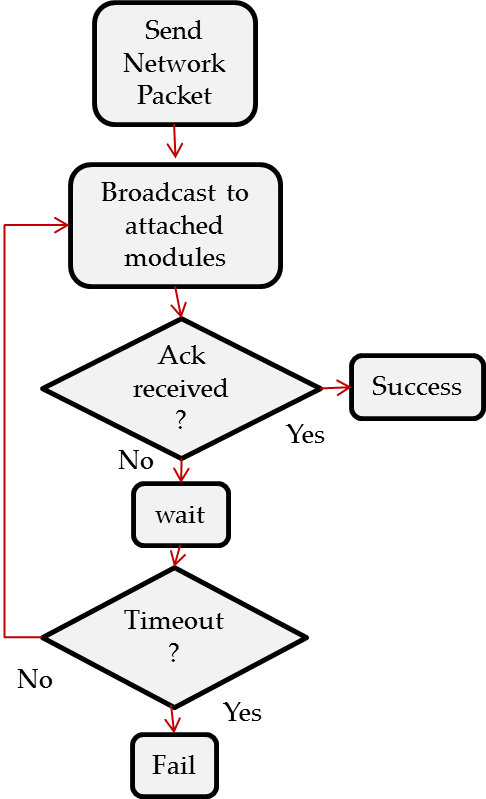
\includegraphics[scale = 0.35]{figures/send_algorithm.png}
\caption{Basic Sending Algorithm}
\label{fig:sending_algorithm}
\end{figure}

Each module has a queue that stores the Packet ID, Source ID and Destination ID of the last N (configurable) network messages received in the module. When a module receives a network packet (identified for a flag in the flags byte) it first checks if the packet is repeated (the packet is present in the aforementioned queue) then discard the packet, otherwise check if the Packet ID byte matches the ID of the module. If the packet is not for the module that received the message broadcast the packet to the attached modules (except for the module that passed the message), if the message corresponds to the ID of the module then make an acknowledgment packet (set the requires global acknowledgment flag in the flags byte to false ) and broadcast it back to the sender module and take the message to the application layer. The figure \ref{fig:receiving_algorithm} exemplifies the receiving network message described.

\begin{figure}[htb]
\centering
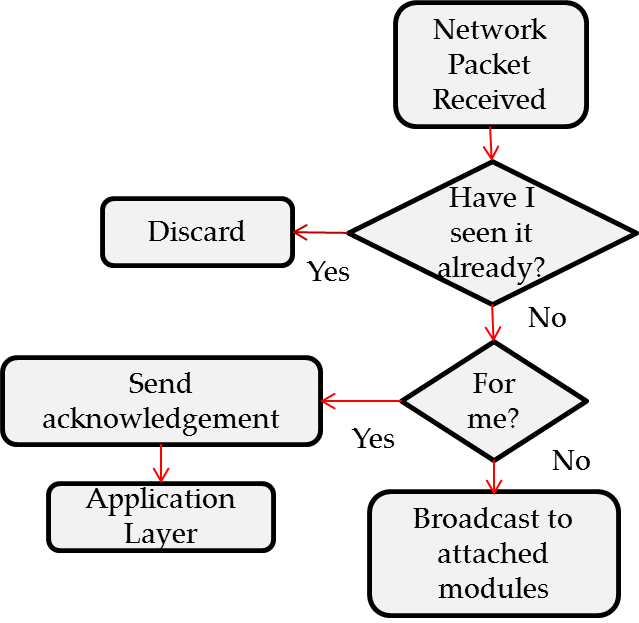
\includegraphics[scale = 0.35]{figures/receive_algorithm.png}
\caption{Basic Receiving Algorithm}
\label{fig:receiving_algorithm}
\end{figure}

\subsection{Application Layer}
 The commands that each module can perform are listed below in the table \ref{tab:command_list}. 
\begin{table}
  {\scriptsize\tt
   \begin{tabular}{| l | l | l | l | l | l | l |  l |}
  \hline
   Command & Byte & Params[1] & Params[2 ] & Params[3] & Params[4] &Params[5] & Params[6]\\ \hline
   {\bf request\_id} & 0x01 & - & - & - &- &- & -\\ \hline
   {\bf return\_id}& 0x02 & MODULE\_ID & - & - &- &- & - \\ \hline
   {\bf request\_routing} & 0x03  & - & - & - &- &- & - \\ \hline
   {\bf return\_routing} & 0x04 & ID[0] & ID[1] & ID[2] & ID[3] & ID[4] & ID[5] \\ \hline
   {\bf network\_acknowledge} & 0x05  & - & - & - &- &- & - \\ \hline
   {\bf move\_top\_servo} & 0x07 & HIGH\_BYTE & LOW\_BYTE  & - &- &- & -  \\ \hline
    {\bf move\_bottom\_servo} & 0x08 & HIGH\_BYTE & LOW\_BYTE  & - &- &- & -  \\ \hline
   \hline
  \end{tabular}
   \caption{Command list}
    \label{tab:command_list}
	}
 \end{table}

The {\bf request\_id} command asks to an attached module to return its ID. The  {\bf return\_id} command returns the ID of the current module to an attached module (that has previously sent a  {\bf request\_id} command), whenever a {\bf return\_id} command is received the module saves the returned ID in a routing table that stored what module is connected to what port. The {\bf request\_routing} command asks to an attached module to return its routing table. The {\bf return\_routing} command returns the routing table of the current module to an attached module (that has previously sent a {\bf request\_routing} command). The {\bf network\_acknowledge} command returns an acknowledgment packet to a specified module (through its ID) on the network. The {\bf move\_top\_servo} and {\bf move\_bottom\_servo} commands move the top or the bottom servomotors in the module to the specified position 



\subsection{Prototyping and Implementation}

The circuits for the robot were implemented in breadboard and tested and also implemented in stripboard (in case that the pcb's did not arrive on time). The result's are shown in the figure \ref{fig:prototype}

\begin{figure}[htb]
\centering
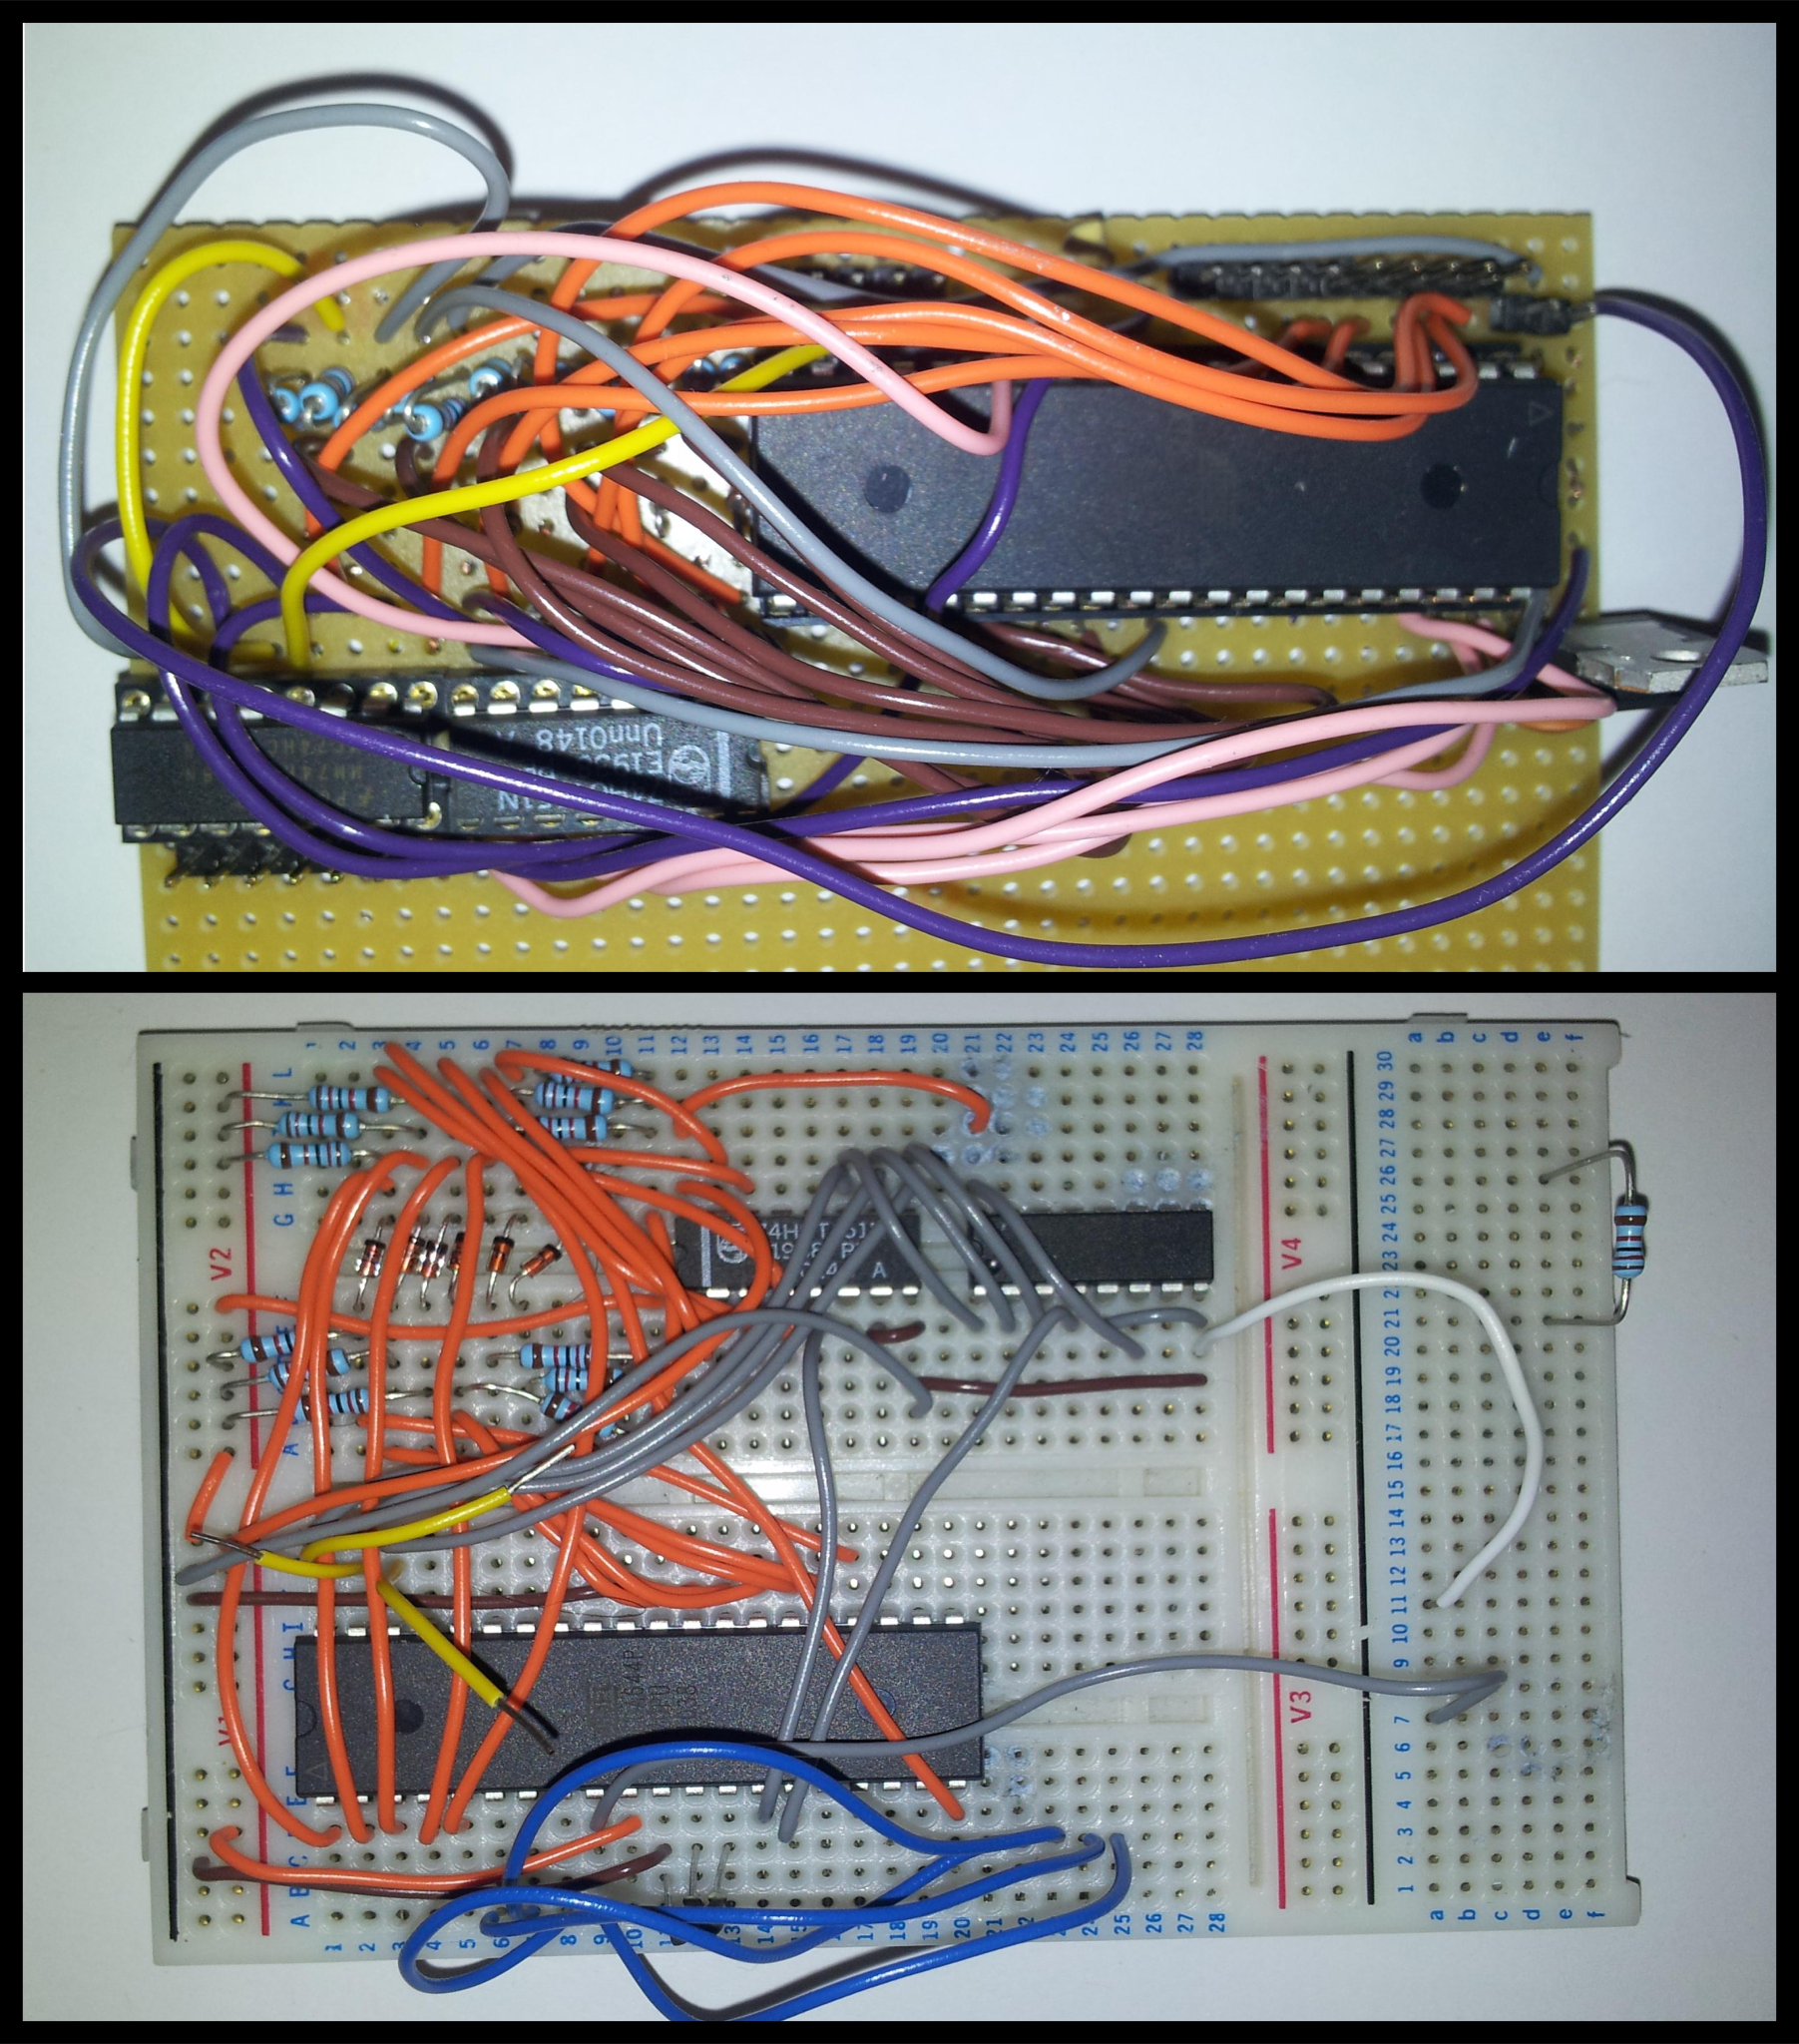
\includegraphics[scale = 0.4]{figures/bred_strip.pdf}
\caption{Proptotypes for the circuit boards of the robot. Done in bread-board (bottom) and the prototype made in strip-board (top)}
\label{fig:prototype}
\end{figure}

After the design was done, one of the biggest problems we faced was the powering of the modules. Only one battery arrived and the charger that we bought could not charge the batteries properly as we expected. We decided to power the modules straight from a DC power supply and made the necessary arrangements on the boards to support this. The problem with using a DC power supply is that requires lots of wiring and long wires between the power supply. This long wires increase the resistance in the circuit ground, when the servo moves a strong peak current passes to the circuit ground and goes through the long wire to the power supply ground as shown in the figure \ref{fig:supply_problem}, therefore the ground in the circuit is lifted and can cause the circuit to reset randomly. With the batteries we would not face this problem because the connection between the circuit ground and battery ground would be short.

\begin{figure}[htb]
\centering
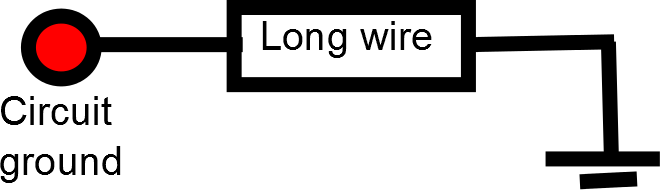
\includegraphics[scale = 0.2]{figures/longwire.png}
\caption{Problem with the power supply connection}
\label{fig:supply_problem}
\end{figure}


